\chapter{Basistechnologien}
\thispagestyle{standard}
\pagestyle{standard}
\renewcommand{\footrulewidth}{0.4pt}
\lfoot{\small Refik Kerimi}

\section{Aufbau PWA}
IN diesem Kapitel werden die Vorteile/Nachteile im Vergleich zu den \acl{NA}s aufgelistet und der Aufbau einer \acs{PWA} erklärt.  

  \begin{figure}[h]
	\centering
	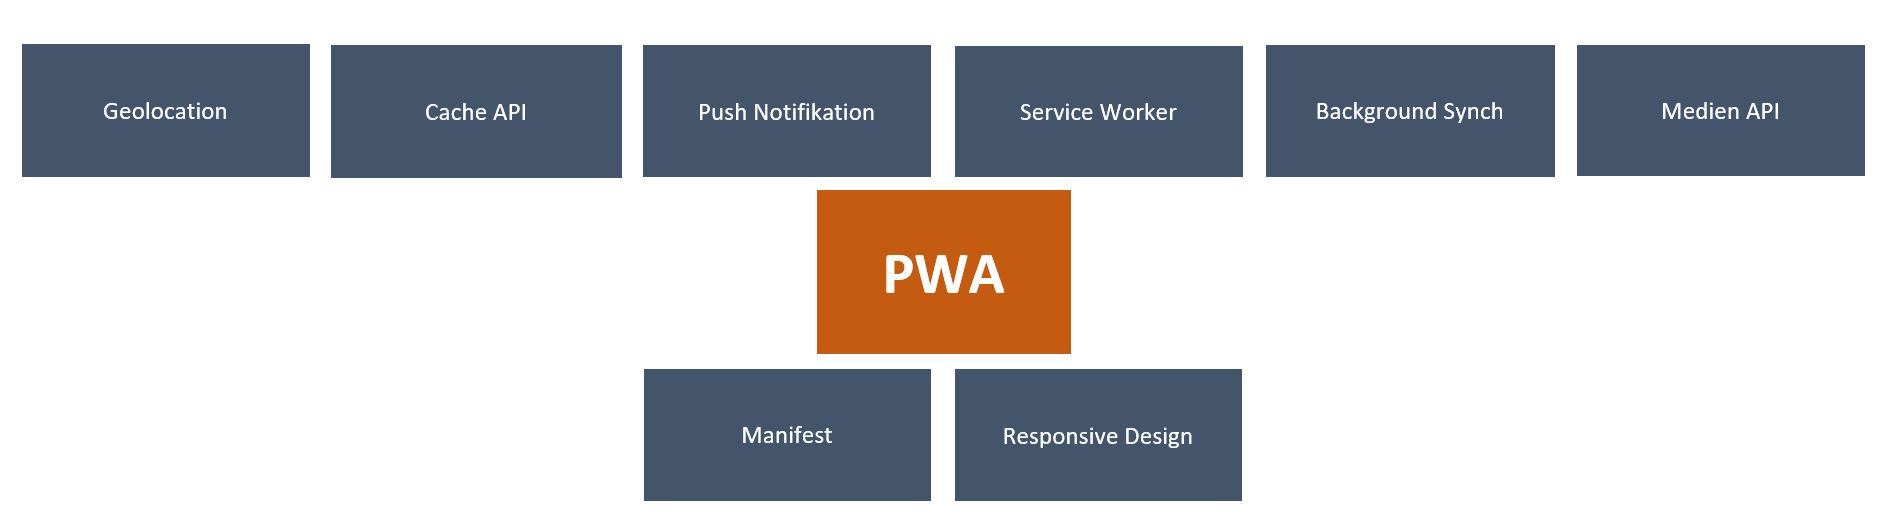
\includegraphics[width=14cm]{BilderAllgemein/PWA_Features}\medskip
	\caption{PWA Komponenten}
	\label{fig:Komponenten}
\end{figure}

\subsection{Tabelle}


%Tabelle verwenden

\begin{table}[h]
\centering
\begin{tabular}{|l|l|l|l|}
\hline\multirow{3}{*}{Firefox 5}
	         &PWA  & Native & 	\\ \hline
   			
   				  & read 		\\	\hline
				1 bit  & read/write \\  \hline
				16 bit & read    	\\	\hline
				16 bit & read/write \\ \hline
\end{tabular}    
\caption{Modbus Datenmodell \cite{ModbusSpecification}}
\label{tab:modbusDataModel}
\end{table}



\section{Web App Manifest}
Das App Manifest ist ein JSON File verrät dem Browser wie sich die \acs{WA}, bei der Installation auf dem Startbildschirm, verhält. Im Manifest wird der Name,der Kurzname, die Größe, Aussehen der Icons und weitere Eigenschaften definiert diese im Kapitel \ref{chap:Entwurf} näher erklärt werden.

\subsection{Verwendung}


\section{Service Worker}
%\label{sec:Service Worker} zuweisung zu anderen Sektor
Der \acl{SW} (\acs{SW}) ist ein Script das der Browser im Hintergrund ausführt \cite{lifecycleSW}. Mit der Hilfe des \acs{SW} ist es möglich die \acs{WA} offline zu betreiben, Push Notifikation zu erhalten, gecachte Daten abzurufen. \acs{SW} verhalten sich wie Proxy-Server, welche in einer Zwischenschicht vom Browser und den Netzwerk sitzen. 
Ein \acs{SW} wird von einem Worker-Kontext \cite{Worker} ausgeführt, hat keinen DOM Zugriff und wird als Haupt-Java Script Thread verwendet \cite{ServiceWorker}.

\subsection{Verwendung}
Der Cyclus eines \acs{SW}s ist von der Webseite getrennt.
In der Installationsphase werden benötigte statische Datein zwischengespeichert erst danach ist der \acs{SW} installiert. Die Installation erfolgt über die JavaScript-Funktion:

\begin{lstlisting}[caption={Service Worker Register},label=lst:ServiceWorkerRegister, xleftmargin=50pt]
navigator.serviceWorker.register
\end{lstlisting}  
Danach folgt die Aktivierungsphase, in dieser Phase werden alte Cache-Inhalte verwaltet und Aktualisiert.
Um die neuen Seiten zu steuern muss der \acs{SW} erneut geladen werden.
In der Abbildung \ref{fig:Erstinstallation} ist eine vereinfachte Erstinstallation zu sehen:

  \begin{figure}[h]
	\centering
	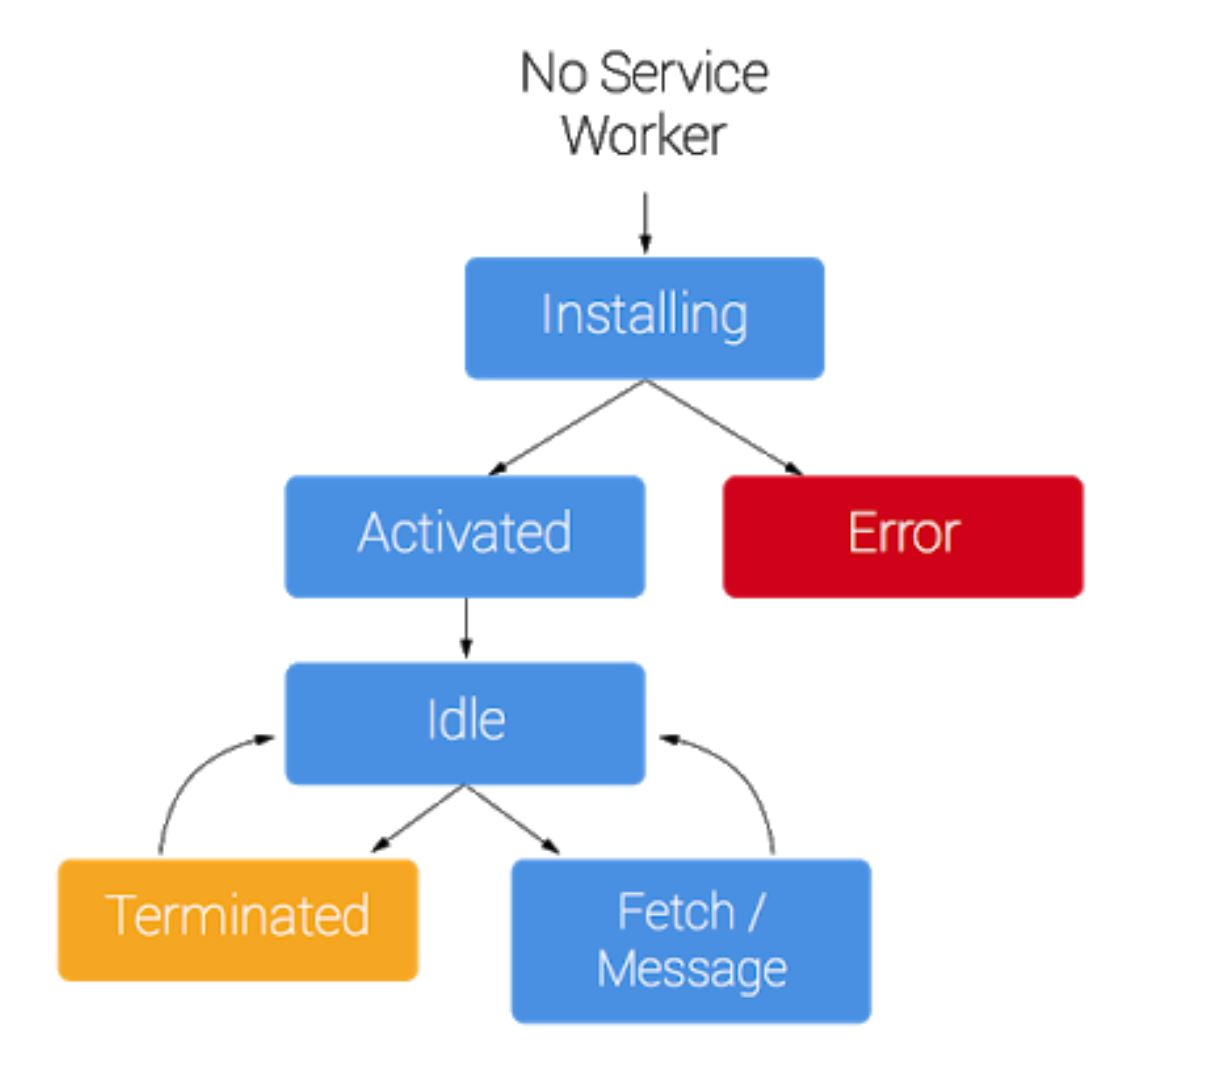
\includegraphics[width=14cm]{BilderAllgemein/InstallSW}\medskip
	\caption{Erstinstallation Service Worker}
	\label{fig:Erstinstallation}\cite{lifecycleSW}
\end{figure}

Der \acs{SW} kann nach der Übernahme der Steuerung zwei Zustände übernehmen, entweder dieser wird beendet oder er übernimmt die Verwaltung der Netzwerkanfragen und der Nachrichten \cite{lifecycleSW}.

\newpage

\subsection{Push Notifikation}
Um dem User bei einer \acs{PWA} das Gefühl einer Native App aufkommen zu lassen ist die Push Funktion unablässig. Erst durch diese Funktion in Kombination mit dem \acs{SW} gibt der \acl{WA} die persönliche Nähe zum User \cite{PushNotifikation}.
\newpage
\subsection{Cache API}

\subsection{Geolocation}
https://appdevelopermagazine.com/5877/2018/3/1/progressive-web-apps-vs-native-apps:-showdown-in-2018/


\subsection{Camera API}


\subsection{Browser} 





\newpage